\documentclass[a4paper,14pt]{extarticle}

\usepackage[top=1in, bottom=1in, left=1in, right=1in]{geometry}
\usepackage[utf8]{inputenc}
\usepackage[russian]{babel}
\usepackage{graphicx}
\usepackage{caption}
\usepackage{subcaption}
\usepackage{chngcntr}
\usepackage{amsmath}
\usepackage{amsfonts}
\usepackage{pgfplots}
\usepackage{pgfplotstable}
\usepgfplotslibrary{fillbetween}
\usepackage{float}
\usepackage{lipsum}% http://ctan.org/pkg/lipsum
\usepackage{multicol}% http://ctan.org/pkg/multicol
\usepackage{hhline}
\usepackage{tabularx}
\usepackage{tikz,xcolor}
\usepackage{tkz-graph}
\usepackage{float}
\usepackage{mathtools}
\usepackage{todonotes}
\usepackage{listings}
\usepackage[makeroom]{cancel}

\usetikzlibrary{arrows, petri, topaths}

\counterwithin{figure}{section}
\counterwithin{equation}{section}
\counterwithin{table}{section}

\begin{document}
\begin{titlepage}
\centering 
{\bfseries Санкт-Петербургский Политехнический Университет} \\
Институт компьютерных наук и технологий \\
Кафедра компьютерных систем и программных технологий \\
\vspace{5cm}
{\centering \textbf{Отчёт о лабораторных работах 4, 5} \\ 
\vspace{0.2cm}
\textbf{Дисциплина}: Телекоммуникационные технологии \\
\vspace{0.2cm}
\textbf{Тема}: Аналоговая модуляция. Частотная и фазовая модуляция.} \\
\vspace{4cm}
\hfill {\bfseries Работу выполнил:}  \\
\hfill гр. 33501/3 Кнорре А.В. \\
\hfill {\bfseries Преподаватель}  \\
\hfill Богач Н.В.
\vfill
Санкт-Петербург \\
{\large 2018}
\end{titlepage}

\section{Цель работы}
\begin{itemize}
\item Изучение амплитудной модуляции и демодуляции сигналов. 

\item Изучение частотной и фазовой модуляции и демодуляции сигналов.
\end{itemize}

\section{Ход работы}

\subsection{Амплитудная модуляция.}

Возьмём за исходный сигнал синусоиду с фазой 90 градусов и периодом $2 * \pi * F0 * t$, где F0 = 5 Гц.

Произведем амплитудную модуляцию с несущей частотой 64 Гц и коэффициентом модуляции M = 0.2:

\begin{figure}[H]
\centering
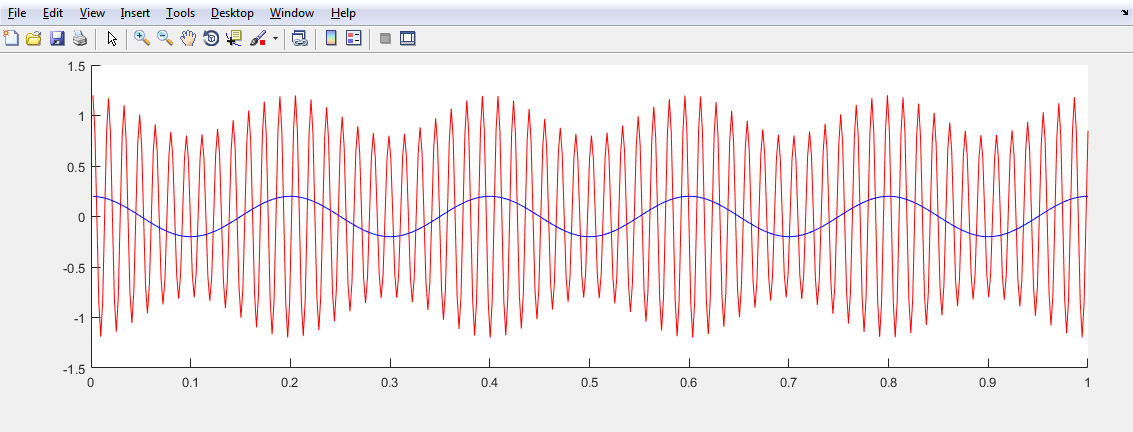
\includegraphics[width=0.95\textwidth]{am}
\captionsetup{justification=centering,margin=1.0 cm}
\caption{Amplitude modulation of input signal}
\label{any}
\end{figure}
На спектре четко видно что частота модуляции отличается от частоты исходного сигнала:

\begin{figure}[H]
\centering
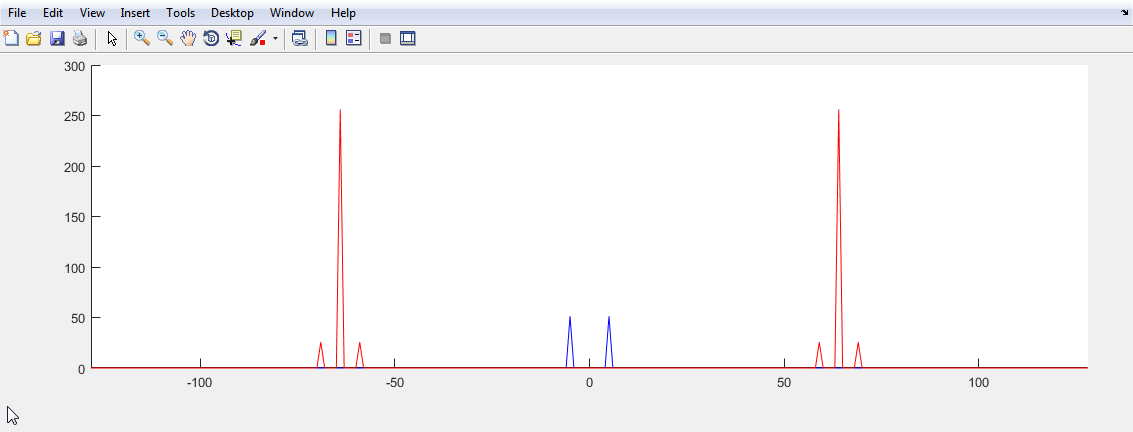
\includegraphics[width=0.95\textwidth]{am_sp}
\captionsetup{justification=centering,margin=1.0 cm}
\caption{Amplitude modulation of input signal' spectrum}
\label{any}
\end{figure}

Произведем демодуляцию и проанализируем увиденное:

\begin{figure}[H]
\centering
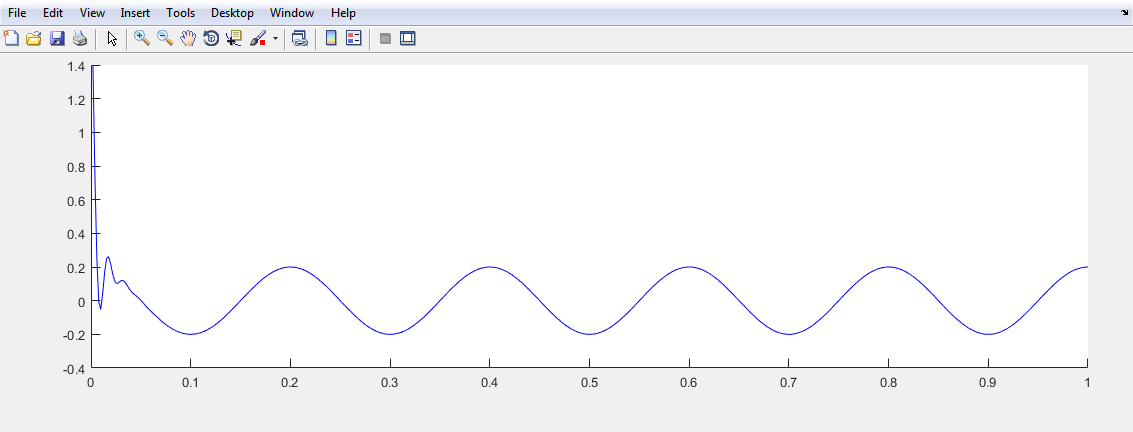
\includegraphics[width=0.95\textwidth]{am_dm}
\captionsetup{justification=centering,margin=1.0cm}
\caption{Demodulation of AM signal}
\label{sig}
\end{figure}
Видны искажения в начале и конце сигнала, связанные с тем, что для демодуляции необходимо накопить некоторое число сэмплов, а также инерционностью данного процесса в конце.

\begin{figure}[H]
\centering
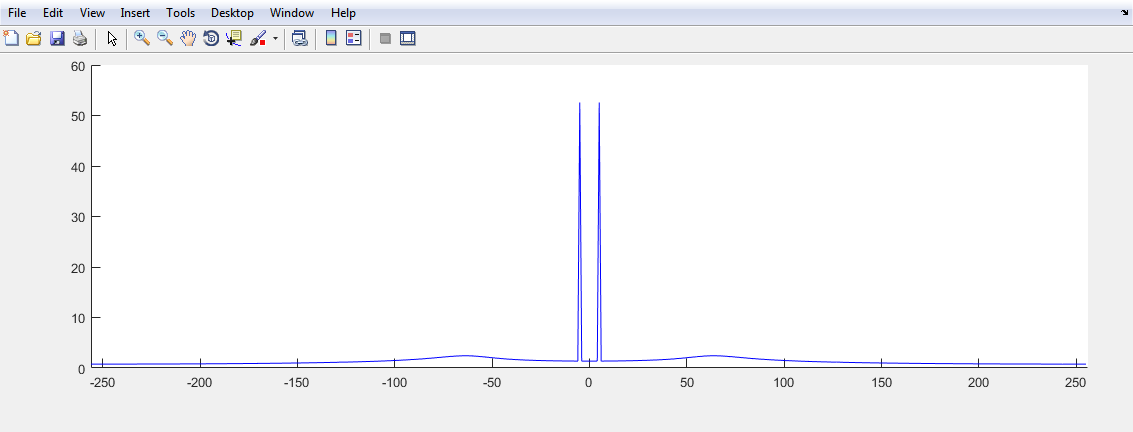
\includegraphics[width=0.95\textwidth]{am_dm_sp}
\captionsetup{justification=centering,margin=1.0 cm}
\caption{Demodulation of AM signal' spectrum}
\label{any}
\end{figure}
Видим что исходная частота сигналов успешно восстановлена с небольшим амплитудным смещением в наблюдаемом диапозоне частот.

\subsection{Частотная модуляция.}

Произведем частотную модуляцию с делителем 8 и несущей частотой 32 Гц.

\begin{figure}[H]
\centering
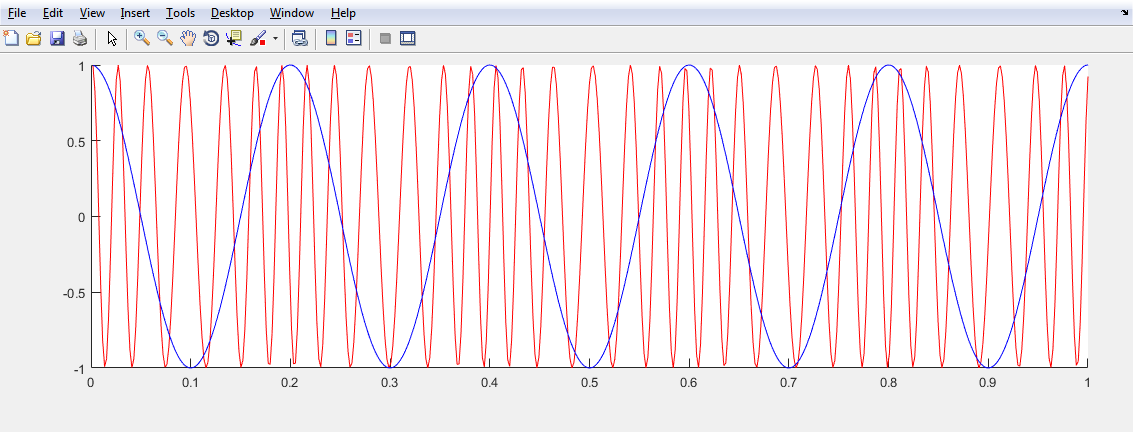
\includegraphics[width=0.95\textwidth]{fm}
\captionsetup{justification=centering,margin=1.0 cm}
\caption{Frequency modulation of input signal}
\label{any}
\end{figure}
Видим что частота сигнала колеблется вместе со значением исходной гармонической функции.

На спектре наблюдаем несущую в 32 Гц и колебания вокруг неё.
\begin{figure}[H]
\centering
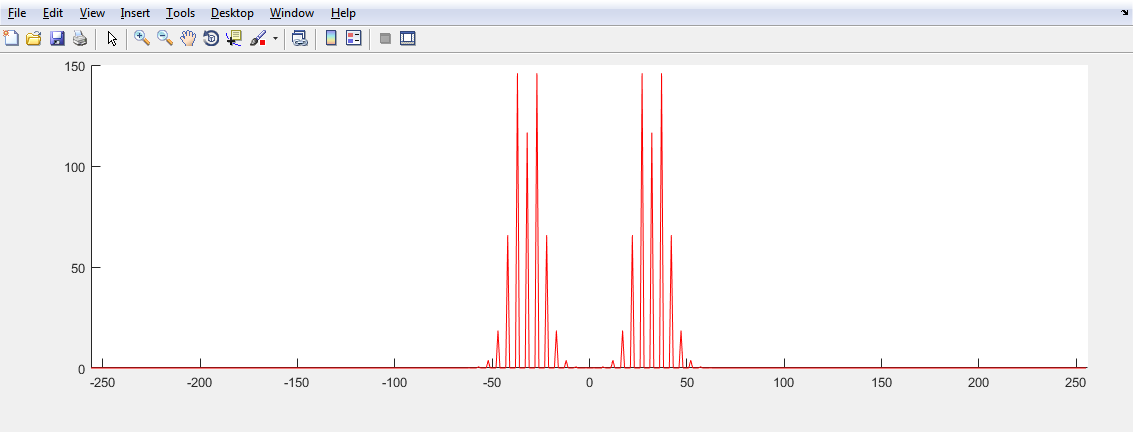
\includegraphics[width=0.95\textwidth]{fm_sp}
\captionsetup{justification=centering,margin=1.0 cm}
\caption{Frequency modulation of input signal' spectrum}
\label{any}
\end{figure}

Произведем демодуляцию и проанализируем наблюдаемое:

\begin{figure}[H]
\centering
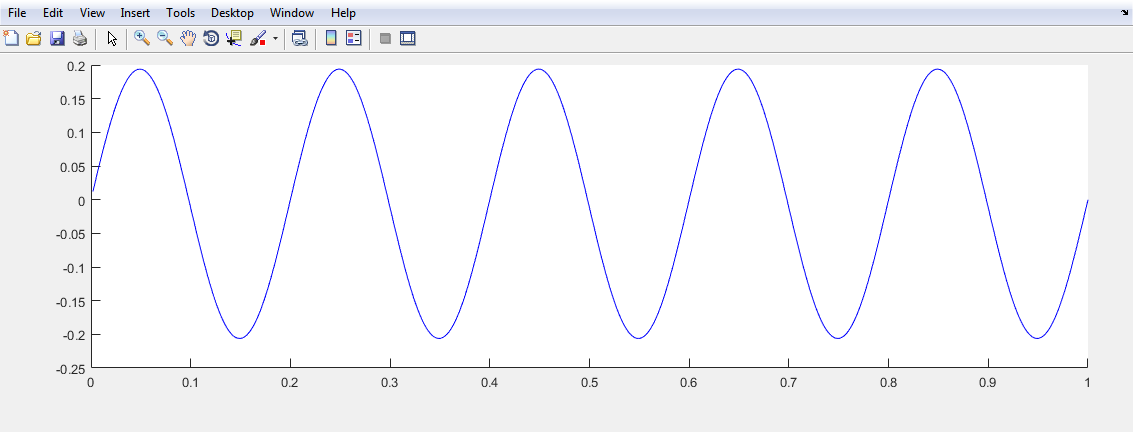
\includegraphics[width=0.95\textwidth]{fm_dm}
\captionsetup{justification=centering,margin=1.0cm}
\caption{Demodulation of FM signal}
\label{sig}
\end{figure}
Видим что при делителе частоты в 8 наш сигнал потерял в амплитуде демодуляции в 5 раз. 

\begin{figure}[H]
\centering
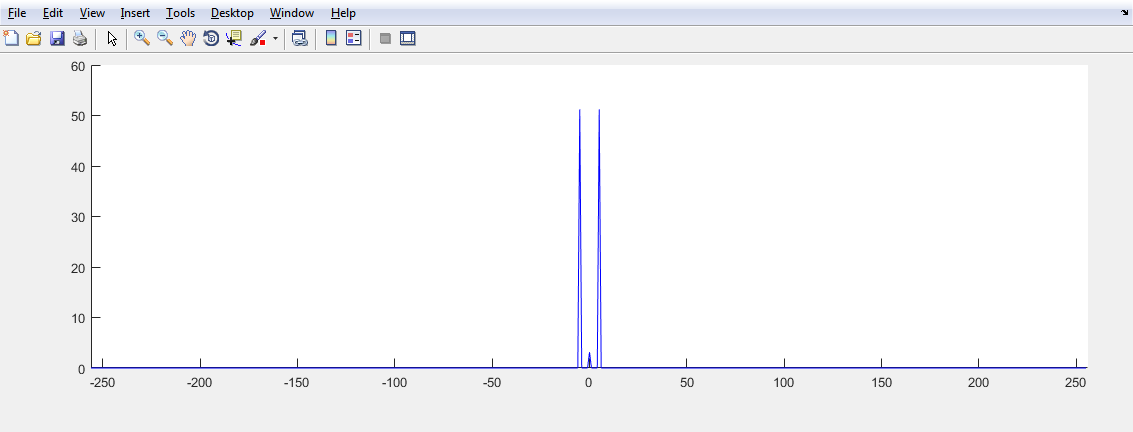
\includegraphics[width=0.95\textwidth]{fm_dm_sp}
\captionsetup{justification=centering,margin=1.0 cm}
\caption{Demodulation of AM signal' spectrum}
\label{any}
\end{figure}
Но частота демодулированного сигнала соответствует исходной в 5 Гц.

\subsection{Фазовая модуляция.}

Произведем фазовую модуляцию с девиацией 1/2.

\begin{figure}[H]
\centering
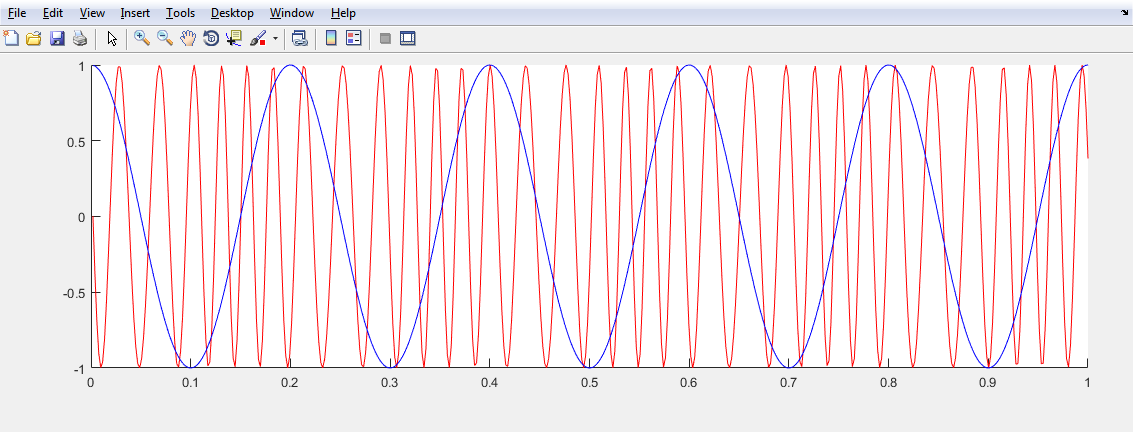
\includegraphics[width=0.95\textwidth]{pm}
\captionsetup{justification=centering,margin=1.0 cm}
\caption{Phase modulation of input signal}
\label{any}
\end{figure}
Видим что фаза сигнала колеблется вместе со значением исходной гармонической функции.

На спектре также наблюдаем несущую в 32 Гц и колебания вокруг неё.
\begin{figure}[H]
\centering
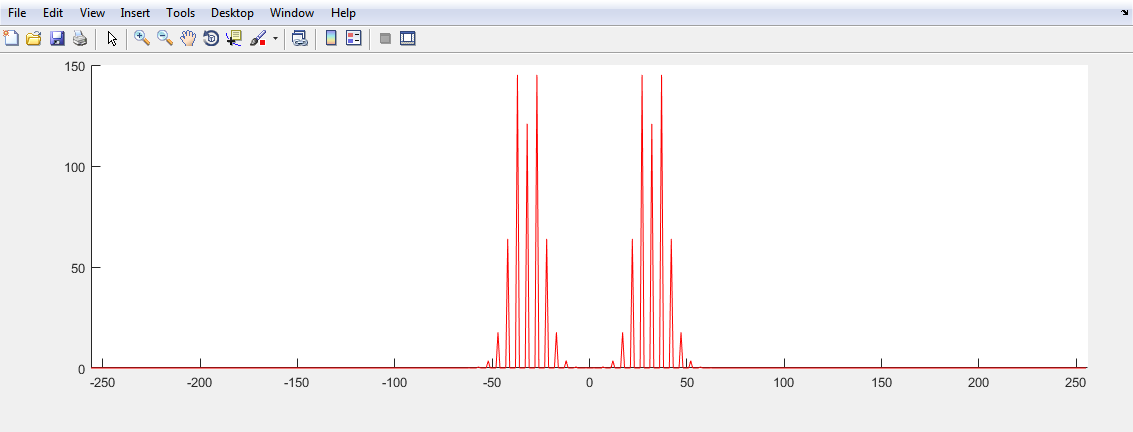
\includegraphics[width=0.95\textwidth]{pm_sp}
\captionsetup{justification=centering,margin=1.0 cm}
\caption{Phase modulation of input signal' spectrum}
\label{any}
\end{figure}

Произведем демодуляцию и проанализируем:

\begin{figure}[H]
\centering
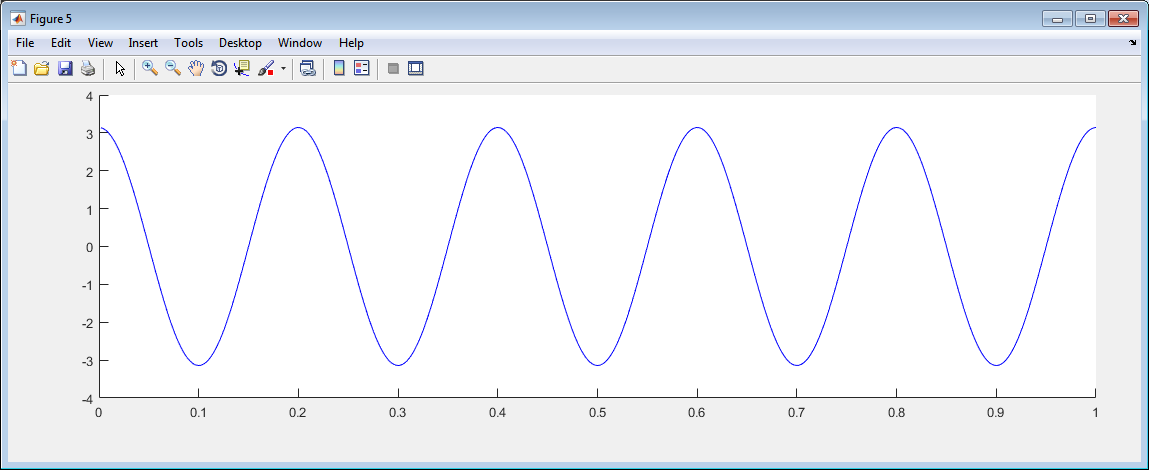
\includegraphics[width=0.95\textwidth]{pm_dm}
\captionsetup{justification=centering,margin=1.0cm}
\caption{Demodulation of FM signal}
\label{sig}
\end{figure}
Видим что амплитуда демодулированного сигнала выросла в 3 раза

\begin{figure}[H]
\centering
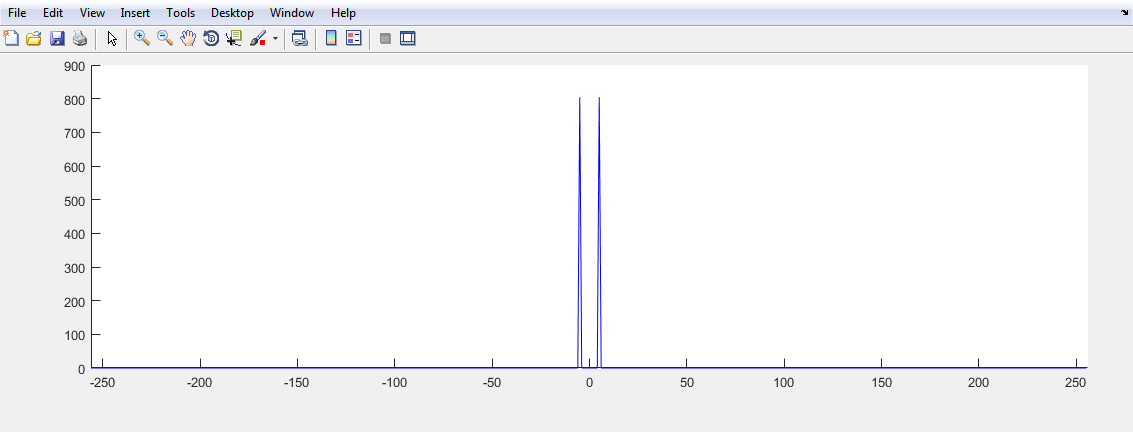
\includegraphics[width=0.95\textwidth]{pm_dm_sp}
\captionsetup{justification=centering,margin=1.0 cm}
\caption{Demodulation of AM signal' spectrum}
\label{any}
\end{figure}
А на спектре, в отличии от частотной модуляции, отсутствуют следы несущей частоты.


\section{Выводы.}

Мы произвели модуляцию и демодуляцию сигнала используя такие параметры гармонического сигнала как:
\begin{itemize}
\item Амплитуду 
\item Частоту
\item Фазу
\end{itemize}

Амплитудная модуляция в наше время применяется всё реже. Однако частотная модуляция встречается довольно часто. 
Радио использует преймущественно частотную модуляцию именно благодаря её преймуществом в помехозащищённости над амплитудной модуляцией.

\end{document}
